\chapter{Mô hình -- Kết quả}
\section{Mạch mô phỏng bằng Protues}
\begin{figure}[h]
\begin{center}
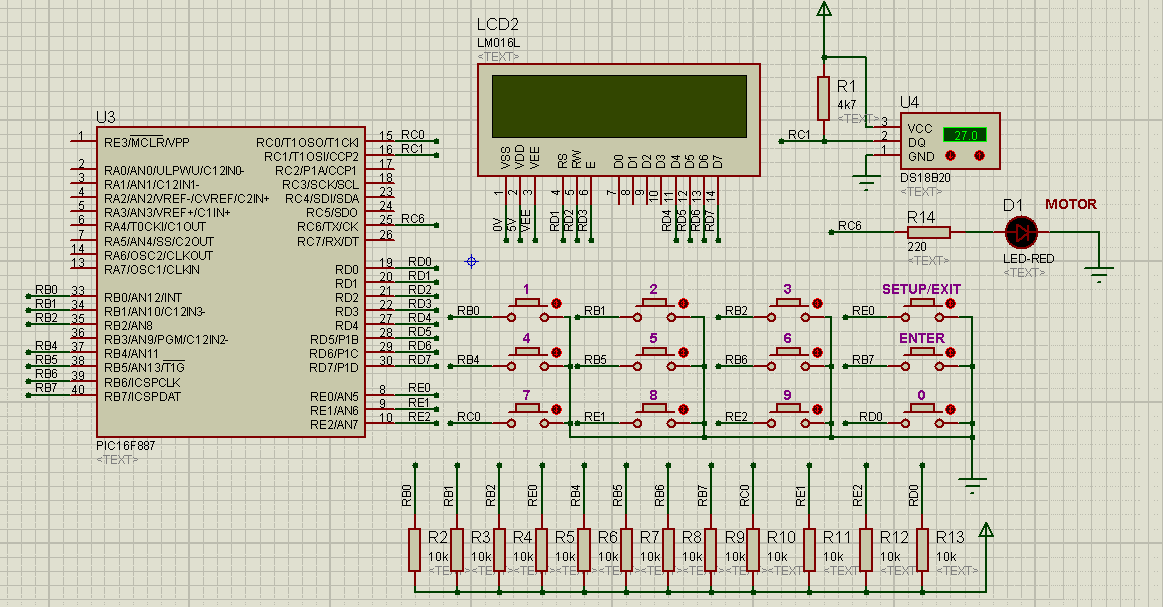
\includegraphics[scale=.5]{MACH_CHINH}
\end{center}
\caption{Mạch mô phỏng của đề tài với Protues}
\end{figure}
\newpage
\section{Kết quả làm mạch thực tế}
\begin{figure}[!h]
\begin{center}
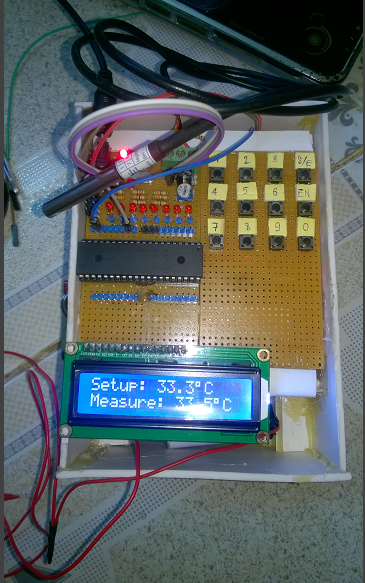
\includegraphics[width=.35\linewidth]{THUC-TE1}
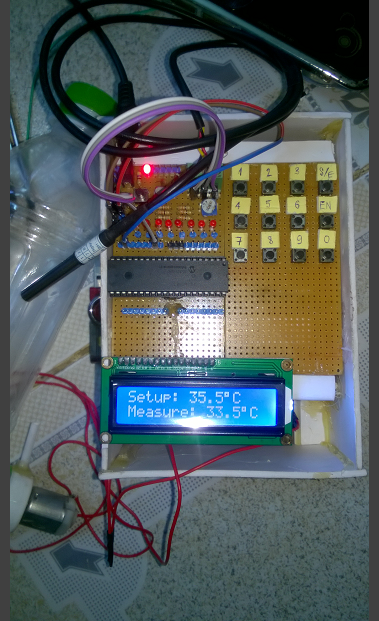
\includegraphics[width=.35\linewidth]{THUC-TE2}\\
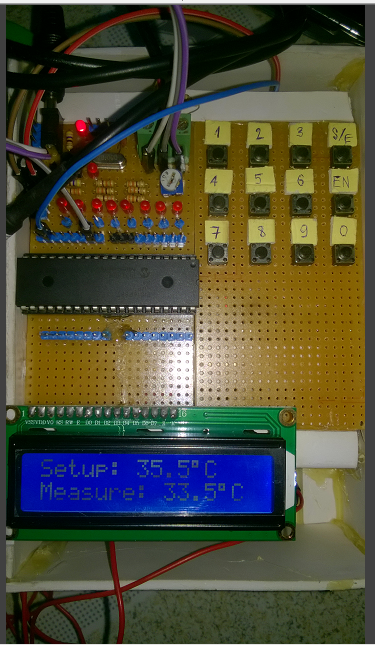
\includegraphics[width=.35\linewidth]{THUC-TE4}
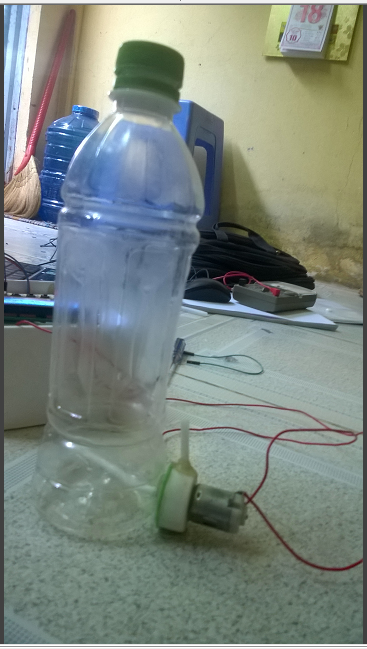
\includegraphics[width=.35\linewidth]{THUC-TE6}
\end{center}
\caption{Mạch làm thực tế của đề tài}
\end{figure}